\documentclass[a4paper,12pt]{article}
\usepackage[T1]{fontenc}	% For use with pdflatex
\usepackage[utf8]{inputenc} % For use with pdflatex
\usepackage[english]{babel}
%\usepackage[estonian]{babel} % Eesti keelsetele lõputöödele

\usepackage{amsmath,amsthm,amsfonts}
\usepackage{graphicx}
\usepackage{listings}
\usepackage[colorlinks=true,linkcolor=blue,urlcolor=blue,citecolor=blue,filecolor=black]{hyperref}
\setlength{\parindent}{0pt} \setlength{\parskip 5pt plus 2pt minus 1pt} \frenchspacing

\newtheorem{theorem}{Theorem}
\newtheorem{corollary}{Corollary}[theorem]
\newtheorem*{definition}{Definition}

%Annika_start
\usepackage[numbers]{natbib}
\bibliographystyle{Chicago_ff}
% increase \bibhang to take care of the numbers (adjust at will)
\setlength{\bibhang}{2pc}
\makeatletter
% patch \@lbibitem to print the current number before the authors
\patchcmd{\@lbibitem}
  {]}
  {]\bbl@box{\theNAT@ctr} }
  {}{}
% add to the aux file the information about the last number
\apptocmd{\endthebibliography}
  {\if@filesw\write\@mainaux{\string\bbl@lastnumber{\theNAT@ctr}}\fi}
  {}{}
% allocate a length, set to a provisional value
\newlength{\bbl@lastnumberwd}
\setlength\bbl@lastnumberwd{0pt}
% this command will be in the aux file and sets the widest label width
\newcommand\bbl@lastnumber[1]{%
  \settowidth\dimen@{[#1]}%
  \global\bbl@lastnumberwd\dimen@}
% a command to print the number
\newcommand{\bbl@box}[1]{%
  \makebox[\bbl@lastnumberwd][r]{[#1]}%
}
\makeatother
\setcitestyle{authoryear,open={(},close={)}}
%Annika_End


\title{Title of the thesis}
\author{Author name}
\begin{document}

% Start with the titlepage
\begin{titlepage}
\begin{center}

\textsc{University of Tartu}\\
\textsc{Faculty of Science and Technology}\\
\textsc{Institute of Mathematics and Statistics}\\[4.5cm]

{\large\textsc{Author}}\\[0.2cm]
{\Large\textsc{\bfseries Title of the Thesis}}\\[0.2cm]
\textsc{Bachelor / Master Thesis}\\[3.2cm]
%\vspace{7.25cm}
\vspace*{\stretch{5}}

{\hfill \sffamily Supervisor: MSc/PhD/prof. Firstname Lastname}

\vspace*{\stretch{8}}

\textsc{Tartu 2020}
\end{center}
\end{titlepage}

% Start page numbers
\pagenumbering{arabic}
\setcounter{page}{1}

% An abstract (in English and Estonian)
\small{

\begin{center}
\MakeUppercase{\textbf{Title of the Thesis}}\\
Bachelor (Master) thesis \\
Author\\
\end{center}

\normalsize{\textbf{Abstract}}\\
Lorem ipsum dolor sit amet, consectetur adipiscing elit. Sed gravida vestibulum venenatis. Cras rutrum facilisis risus ac efficitur. Praesent et lorem massa. In quis suscipit velit. Donec sollicitudin nisi a sem tempor varius. Vestibulum tincidunt lectus nunc, et lacinia orci vulputate ut. In mollis nisl purus, eu congue sem congue non. Fusce fermentum consectetur accumsan. Praesent viverra velit eget sagittis aliquam. Integer non euismod lectus. Nam eget risus quis tellus volutpat varius eu at massa. Suspendisse dignissim commodo rhoncus. Curabitur et dui quis est hendrerit tempor in at lacus. Etiam eu lorem imperdiet, vehicula nunc et, blandit mauris. Praesent dictum rutrum mi, sit amet sodales lacus auctor et. In sagittis augue imperdiet sagittis feugiat.\\
\textbf{CERCS research specialisation:} P160 Statistics, operations research, programming, financial
and actuarial mathematics.\\
\textbf{Key Words:} Random, sample, probability.\\
}

\vspace{0.5cm}

\small{

\begin{center}
\MakeUppercase{\textbf{Lõputöö pealkiri}}\\
Bakalaureusetöö (Magistritöö)\\
Autor\\
\end{center}

\normalsize{\textbf{Lühikokkuvõte}}\\
Lorem ipsum dolor sit amet, consectetur adipiscing elit. Sed gravida vestibulum venenatis. Cras rutrum facilisis risus ac efficitur. Praesent et lorem massa. In quis suscipit velit. Donec sollicitudin nisi a sem tempor varius. Vestibulum tincidunt lectus nunc, et lacinia orci vulputate ut. In mollis nisl purus, eu congue sem congue non. Fusce fermentum consectetur accumsan. Praesent viverra velit eget sagittis aliquam. Integer non euismod lectus. Nam eget risus quis tellus volutpat varius eu at massa. Suspendisse dignissim commodo rhoncus. Curabitur et dui quis est hendrerit tempor in at lacus. Etiam eu lorem imperdiet, vehicula nunc et, blandit mauris. Praesent dictum rutrum mi, sit amet sodales lacus auctor et. In sagittis augue imperdiet sagittis feugiat.\\
\textbf{CERCS teaduseriala:} P160 Statistika, operatsioonianalüüs, programmeerimine, finants- ja kindlustusmatemaatika.\\
\textbf{Märksõnad:} Juhuslik, valim, tõenäosus.\\
}

% Print out the table of contents
\tableofcontents

% Structure of the thesis, each part is set in a separate .tex file
\section*{Introduction}
\addcontentsline{toc}{section}{Introduction}  

The main text of a thesis always starts with an ``Introduction''.
You can leave writing it to the final phase of writing.

It is a good idea to start the Introduction with the main thesis
statement or research question of the thesis.  After that, it is a
good idea to clarify things by defining any necessary
terms.\footnote{Definitions after the thesis statement!  Also, don't
  babble in the introduction.}  This section is also a good place
to discuss why your thesis statement is scientifically or practically
relevant and interesting. Introduction is the place where you explain what is 
your contribution -- knowledge that you have investigated or produced 
personally. At the end of the section, it is customary to briefly
explain the structure of the thesis -- what each chapter is about.

Please note that the instructions given in this sample are by no means
official.  Always follow your supervisor's instructions even if they
conflict with what this sample says.
\section{The structure of the thesis}

There should be 5--8 numbered chapters in a thesis, including
Introduction and Conclusion.  If necessary, you can use sections
and subsections to give the thesis a more fine-grained structure.

The chapters that lie between Introduction and Conclusion are 
collectively called the \textit{body} of the thesis.  It is
often said to start with a \textit{theoretical part}, which is then
followed either by a \textit{main theorem}, a \textit{constructive part}
or an \textit{empirical part}.

\subsection{The theoretical part}

The goal of the theoretical part of a thesis is to develop the
theoretical background required in the thesis.  The idea is that a
reader of the thesis should be able to understand all the special 
concepts and methods used in the thesis.
A good thesis also gives well-argued reasons for why exactly these
concepts and methods are in use in the thesis (with the main
alternatives given in the literature mentioned).

The best way to present and use of the theoretical background depends on
what the thesis is about. The theoretical part of a
fully mathematical work differs considerably from the theoretical part of a quantitative or qualitative
empirical study. 

Some suggestions:
\begin{itemize}
\item In a fully mathematical (theoretical) thesis this chapter usually introduces the 
mathematical background, general theory that is the setting of your contribution.
\item In an empirical thesis it is usually chapter where you describe the 
methodology or explain the method(s) you will use to address the main problem 
of your thesis.
\end{itemize}

Reading other thesis of the same type will give you a good impression
of what is required of your own thesis.

\subsection{Main contribution}

The theoretical part is followed by your contribution:
\begin{itemize}
\item In a fully mathematical (theoretical) thesis it is usually a sequence of
  definitions and lemmas of your own devising, which then culminate in
  the proof of your main theorem.
\item In a constructive thesis it is usually a computer program, algorithm or
  other artefact that you have made yourself.
\item In an empirical thesis it is a set of empirical results obtained
  by applying a empirical research method.
\end{itemize}

You should present your contribution with precision, giving reasons
for the choices you have made.  You should follow the best practices
of the research tradition you are using.
\section{Formatting}  

A thesis is written with a single-column layout on one- or two-sided
A4 sheets. The font type of the body text is usually Times New Roman 
and the font size is 12 pt. The text is fully justified and hyphenated.
You do not have to indent the paragraphs.

\subsection{Mathematical notations}

Numbers are generally written using numerals for the sake of clarity,
for example ``6 stages'' rather than ``six stages''. You should
also use a thousand separators\footnote{Use tilde \~{} in LaTeX and a
  special character \textit{non-breaking space} in MS Word},
i.e. instead of 55700125 write 55~700~125. Never omit the leading zero
in decimals. For example, it is correct to write ``0.5'' and wrong to
write ``.5''. A comma is used as a decimal separator in the Estonian
language and a period in the English language.

Like numbers, it is advisable to abbreviate units of
measurement. There is a space between the number and the unit, but you
should keep them on the same line. It is better to compile a table or
graph than include a great deal of numerical values in the body
text. Use precise language and put numbers on a scale.

Newton's Second Law can be presented in the following way:

\begin{equation}
  \label{eq:newton2}
 F = ma,
\end{equation}

where $m$ denotes the mass of an object, $a$ means acceleration, and
$F$ means force. Please note that all the variables must be defined at
the point of their first appearance. All sentences end with a
punctuation mark, and the main elements of a sentence are separated by
a comma in accordance with the rules of English grammar. Consider formulas 
as part of a sentence, therefore use commas or period accordingly after 
formulas (e.g. see equation (\ref{eq:newton2})).

Formulas can be numbered or not numbered. Numbered formulas are used if there is need to refer to these formulas later on. For example, let us have a formula
\begin{equation}\label{eq:pythagoras}
c^2=a^2+b^2.
\end{equation}
Then, since \eqref{eq:pythagoras} is numbered, we can always refer to it in later text. For example, specifying $a=3$ and $b=4$ and applying \eqref{eq:pythagoras} implies $c=5$.

On the other hand, if we do not refer to some formula or equation at all, it should not have a number, for example:
\[
S_n=\sum_{i=1}^n X_n.
\]

Occasionally mathematical notations are preceded by an
identifier, such as 'Definition 1' or 'Theorem 1'. Simple formulas may 
be displayed within the body of the text without numbering.

Please note that usually different styles applied to same letter/symbol refer to different object, for example, $x$, x, $X$, \textit{\textbf{X}}, $\mathbf{X}$, ..., are all different. Also, a general rule is that variables are in italic and function names are in regular font, for example, $s$, $u$ and $p$ are some variables, and supremum function $\sup$ is in regular font so we do not confuse it with the product $sup=s\cdot u\cdot p$. 

Please try to use unified notation (i.e. same letter/symbol should mean the same variable or function) throughout the whole document (as much as possible).


LaTeX is the best editor for writing also the more complex equations, such as
\begin{equation}
  \label{eq:fourier}
  G^+(t,t')= \int G^+(E) \exp[-iE(t-t')/\hbar] dE.
\end{equation}

\subsection{Theorems and definitions}

Mathematical thesis often include elements that require special formatting and numbering such as theorems, definitions, propositions, remarks, corollaries, lemmas and so on. Such formatting can be achieved by defining special environment with the \verb+\newtheorem+ command in the preamble of the document. For example:

\begin{theorem}
Let $f$ be a function whose derivative exists in every point, then $f$ is 
a continuous function.
\end{theorem}

\begin{proof}
If a derivative of function $f$ exists in point $x_0$ (meaning that $f$ is differentiable at point $x_0$), then $f$ is continuous at point $x_0$ (differentiability implies continuity - not proven here). 

Assume that function $f$ is differentiable in every point, then that implies that $f$ is continuous at every point and $f$ is a continuous function.
\end{proof}

For the next theorem we need a definition:

\begin{definition}
A right triangle is a triangle in which one angle is a right angle (that is, a 90-degree angle).
\end{definition}

Notice that the definition does not have a number. This can be achieved by defining the definition environment with the \verb+\newtheorem*{}+ command.

\begin{theorem}[Pythagorean theorem]
\label{pythagorean}
This is a theorem about right triangles and can be summarised in the next 
equation 
\[ x^2 + y^2 = z^2 \]
\end{theorem}

And a consequence of Theorem \ref{pythagorean} is the statement in the next 
corollary (you can reference theorems when a label is assigned).

\begin{corollary}
There's no right rectangle whose sides measure 3cm, 4cm, and 6cm.
\end{corollary}

Notice that the Corollary has different numbering, this is because the environment is defined with \verb+\newtheorem{corollary}{Corollary}[theorem]+ , where the square brackets determines the environment that will be used for numbering (also refered to as counter). The same logic can be applied to formulas and theorems, if there are many of such elements. Often the counters are determined by section, for example "Theorem 2.3" refers to the 3rd theorem in the 2nd section of a document. 

By default, each theorem uses its own counter. However it is common for similar types of theorems (e.g. Theorems, Lemmas and Corollaries) to share a counter. In this case, define subsequent theorems as:
\begin{verbatim}
\newtheorem{<name>}[<counter>]{<Printed output>}
\end{verbatim}
where counter is the name of the counter to be used.


\subsection{Figures}

You must refer to all the figures in the body text. The reference
should preferably appear on the same page as the actual figure or
before it (e.g. Figure~\ref{fig:ex_fig}). Figures and tables must be numbered consistently thesis
and primarily placed at the top of the page, but you are free to
decide where they fit best. Never start a chapter with a figure, table
or list.
% Note: put tilde between text and ref command, like in
% 'Figure~\ref{fig:ex_fig}' above. Tilde (~) puts a white space but
% prevents line break. Same thing applies to Table~\ref{tab:summary}
% as well.

Figures and the caption are consistently centered  and the caption is 
placed under the figure and always on the same page as the figure. 
All figures must be explained in the body text, so that readers know 
what they are supposed to notice. 

The figures should be in the same language as other text. The recommended 
font size is the same as that of the body text but no smaller than 10 pt. 
The figures must be readable, even if your thesis is printed in grey-scale!

% Here's an example how to add a figure. Default placement of figures
% is at top of page, i.e. placement specifier is '[t]' could be
% omitted.  The dimensions can be relative to text width (or height)
% or absolute (4 cm).

\begin{figure}[t]
  \begin{center}
    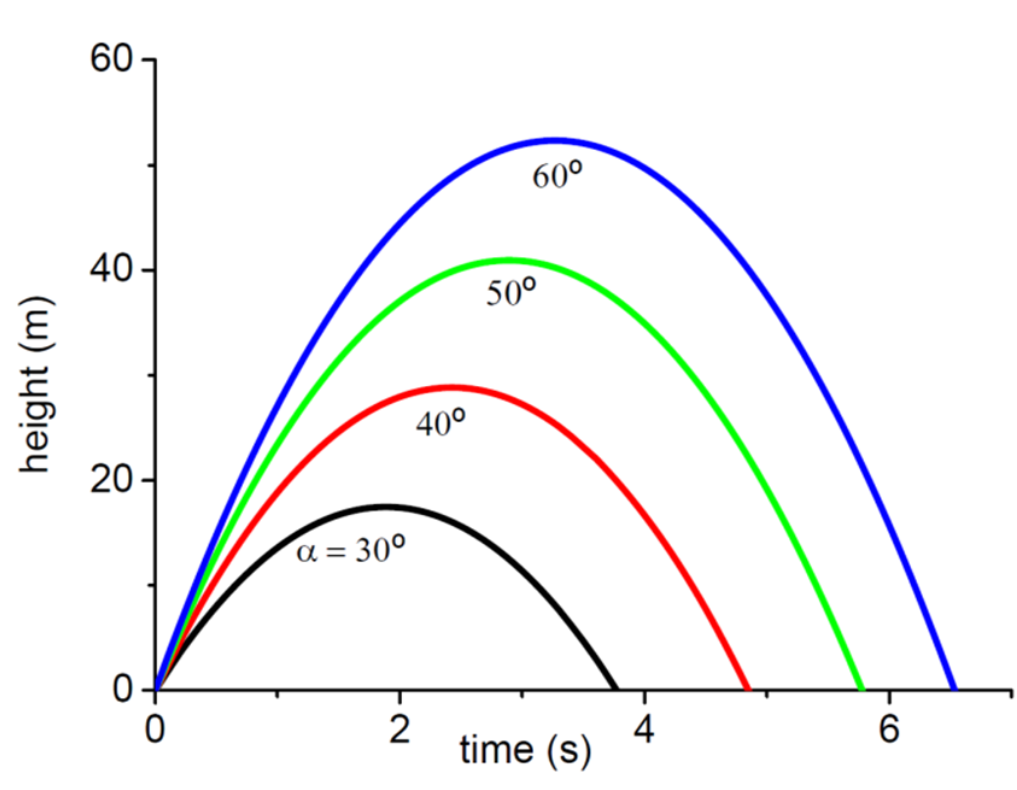
\includegraphics[width=0.7\textwidth]{figure}
  \end{center}
  \caption{Diagram of achieved height and time of flight with different angles of release.}
  \label{fig:ex_fig}
\end{figure}


\subsection{Tables}

Tables have numbered captions, see Table\ref{tab:thin_film} for
example. The caption is placed on the same page above the table. You 
must refer to all the tables in the body text. In addition, you must 
discuss the content of any tables in the body text to ensure that readers 
understand their relevance.

\begin{table}[ht]
  \small
  \begin{center}
    \caption{Example of evaporation conditions in a thin film structure.}
    \label{tab:thin_film}
    \begin{tabular}{l | r r r r r}
      % l = align to left (e.g. text), c=align to center, r=align to
      % right (e.g. numbers), Pipe | creates vertical line
      % Let's put 1 horinzontal line above the table, 2 after header rows,  and 1 below
      \hline
      \textbf{Substance} & \textbf{Thickness}& \textbf{Correction } & \textbf{Pressure}  & \textbf{Current} & \textbf{Speed} \\
                         & \textbf{(nm)}     & \textbf{coefficient} & \textbf{(mbar)}    & \textbf{(mA)}    & \textbf{(nm/s)} \\
      \hline 
      SiO$_2$	& 181.0	& 1.10	& $3.0\cdot10^5$	& 20-23	 &0.2 \\
      TiO$_2$	& 122.1	& 1.55	& $1.5\cdot10^4$	& 100-93 &0.1 \\
      \hline
    \end{tabular}
  \end{center}
\end{table}


Often it is better to create the table in, e.g. MS Excel, and import
it as .eps or .pdf file, for example, when you calculate some of the
values automatically.
%\begin{table}[h]
%  \begin{center}
%    \caption{Example of evaporation conditions in a thin film structure.}
%    \label{tab:thin_film_graphics}
%    \includegraphics[width=8cm]{my_table.eps}
%  \end{center}
%\end{table}

You can use boldface to highlight the header row. Do not surround all 
the cells with a border, as it may make your table harder to read. 
Put a line on top and bottom of the table. You can add a horizontal line
grouped into categories.

The numbers are right aligned (optimally lined up at the decimal
point) for easy comparison. You should preferably use SI units,
established prefixes and rewrite large numbers so that the power of
ten should be placed in the title of the column instead of each row,
if possible. 


\subsection{Programs and algorithms}

Codes and algorithms are written using mono-spaced font, such as
Courier New, Consolas or their variations. If the length of the code
or algorithm is less than 10 lines and you do not refer to it later on
in the text, you can present it similarly to formulas.  Here's an
example showing a snippet (install package \verb!listings! for coloring your code according to type):

\begin{verbatim}
\begin{lstlisting}[style=console, % title={Template files} ] 
all: ${TARGET}.tex
	pdflatex ${TARGET}.tex
	bibtex ${TARGET}
	pdflatex ${TARGET}.tex
\end{lstlisting}  
\end{verbatim}


If the code is longer but shorter than a page, you present like a
figure (Program 4.1) titled ``Program'' or ``Algorithm''.
You should add some comments to the code and indent it
consistently. The actions performed by the code must be outlined in
broad terms in the body text. Line numbers make it much easier to
refer to the code in the text. 

LaTeX has a packages that enable automatic code formatting like
highlight reserved words, bring out string input or color comments differently.
\section{Using references}

This section will give an overview on how to use references. But first, a little more about structure. Pay notice that there should always be an introductory part to the whole chapter. If a chapter headline is immediately followed by a subsection, then this is considered bad practice. Having some text between headlines also makes your thesis more pleasant to read. See \nameref{background} section for more.

\subsection{References and citation}

The list of references is the last section of the document. References can be ordered in alphabetic order (preferred) or in order of citation. The references section of this document covers three most common types of resources and also has some examples. 
The style of formatting of references provided in this document is recommended, but not mandatory. The key points to remember are that 
\vspace{-2mm}
\begin{itemize}
\item all the relevant information about a resource should be included;
\item references of same type should be formatted using same style (e.g., all books have their style, articles their style, etc.).
\end{itemize}

The most common citation style is via the last name(s) of the author(s) and the year of publication (also known as Chicago style referencing). For example, if this sentence is taken from the first reference in the list (see the last section), it can be referred to as (Articleauthor, year). If a whole paragraph needs reference to the same resource, it can simply be added to the end of the whole paragraph, as is done with the second reference. (Bookauthor et al., year)

Furthermore, if a whole section or subsection needs reference(s) then this can be specified in the beginning of this section or subsection. For example, one may say something like "\textit{We refer to Bookauthor et al. (year) and Bookauthor2 \& Bookauthor (year) for the results of this section.}". 

For a complete guide on Chicago style referencing see: \href{http://libguides.library.curtin.edu.au/referencing/chicago}{Chicago 17th B (Author-Date) referencing guide}


\subsection{Using literature}

The theoretical part is almost always based solely on the literature.
When discussing your contribution, you may also need to cite some 
known results in literature.

Remember to avoid plagiarism!  If you copy, either verbatim or with
slight changes (or, example, in your own translation) text from some
source, make it clear to the reader.  Mark your quotes (using
quotation marks or some other clear manner) and give a precise
citation.  If you do not quote verbatim, mark any changes you have
made.  In most situations, however, it is better to use your own
words, based on more than one source.  Even then, give clear
citations.

This guidelines document uses the \textsc{Bib\LaTeX}
system \parencite{biblatex-manual} and Chicago
style \parencite{biblatex-chicago-manual}.  You can switch off this
automation by using the \string\documentclass-option manualbib, but
that means you have to take care of the bibliography yourself, and the
techniques discussed below may not be available. See Appendix 2 for 
information on manual bibliography. Please note that the
Institute recommends using a Chicago style for your bibliography. 
% MIS STIILI SOOVITAME?

\subsection{Citations}

You can cite sources in two ways.  First, you can use the citation as
a noun: \textcite[Chapter~8.8.4]{aho-compilers} briefly discuss the
use of graph coloring in the register allocation phase of a compiler.
In this case, use the \string\textcite\ command.  Second, you can use
a citation as a parenthetical, which is not read aloud: Graph coloring
is one possibile way to allocate
registers \parencite[Chapter~8.8.4]{aho-compilers}.  Use the
\string\parencite\ command for this.

Both commands (\string\textcite\ and \string\parencite) take three
parameters, two of which are optional.  The first (optional) parameter
is a pre-note, the second (optional) parameter is a post-note, and the
third (mandatory) parameter is the citation
key \parencite[see][Section~3.7]{biblatex-manual}.  The citation in
the preceding sentence was made using the following command:

\begingroup\footnotesize
\begin{verbatim}
\parencite[see][Section~3.7]{biblatex-manual}
\end{verbatim}
\endgroup

If you give these commands just one optional argument (that is, one
enclosed in square brackets), it will be interpreted as a post-note.
If you want to give only a pre-note, leave the post-note empty
\parencite[see][]{biblatex-manual}:

\begingroup\footnotesize
\begin{verbatim}
\parencite[see][]{biblatex-manual}
\end{verbatim}
\endgroup

It is also possible to cite multiple sources in the same citation
%
\parencites%
  [see][Section~3.7]{biblatex-manual}%
  [regarding citations in general, see also][Section~5.3.2]%
    {biblatex-chicago-manual}%
\relax.
%
Use the command  \string\parencites\
for this.  For each citation, give it the same parameters as you would give
a single \string\parencite\
command.  It is good practice (but often not necessary) to end the command
in a \string\relax, so that no surprises ensue.

\begingroup\footnotesize
\begin{verbatim}
\parencites%
  [see][Section~3.7]{biblatex-manual}%
  [regarding citations in general, see also][Section~5.3.2]%
    {biblatex-chicago-manual}%
\relax.
\end{verbatim}
\endgroup

If you break the command into multiple lines, use the comment sign
to end each line, to prevent spurious spaces.

Some more examples on how to format citations:

Command: \verb|\citep[see, \textit{e.g.},][]{FreesValdez2008}|\\
Result: \citep[see, \textit{e.g.},][]{FreesValdez2008}

Command: \verb|\cite{HastieTibshiraniFriedman09,DeJongHeller2008}|\\
Result: \cite{HastieTibshiraniFriedman09,DeJongHeller2008}

Command: \verb|\citep{HastieTibshiraniFriedman09,DeJongHeller2008}|\\
Result: \citep{HastieTibshiraniFriedman09,DeJongHeller2008}

Command: \verb|\citep[see, \textit{e.g.},][]{DeJongHeller2008}|\\
Result: \citep[see, \textit{e.g.},][]{DeJongHeller2008}

Command: \verb|\citep{Kim2013bayesian}|\\
Result: \citep{Kim2013bayesian}

Command: \verb|\parencite{Kim2013bayesian}|\\
Result: \parencite{Kim2013bayesian}


Command: \texttt{\citep{cizek_etal}, \citep{hogg_klugman}}\\
Result: \citep{cizek_etal}, \citep{hogg_klugman}


\section*{Conclusions}
\addcontentsline{toc}{section}{Conclusions}  


The last chapter of a thesis is the Conclusions (some authors use
Conculsion, instead).  Keep it short, and discuss what one can
conclude about the thesis statement or research question given in the
Introduction, in light of all that has been written in the thesis.
The Conclusion is also the place to discuss any limitations and
weaknesses of the thesis (especially those that cast doubt on the
reliability of the results given in the thesis), if they have not been
already discussed, for example in a Discussion chapter.  It is also
customary to state, what further research might be beneficial in light
of this thesis.

If the Conclusions threatens to become too long, it is a good idea to
split the interpretation of the results into its own chapter, often
called Discussion, making Conclusions short and sweet.

After Conclusions, there is the bibliography.

% Add the bibliography using the BibTeX functionality. 
%  For manual bibliography see Appendix 2
\pagebreak
\addcontentsline{toc}{section}{List of references}
\printbibliography

% KAS MUU KEELNE KOKKUVÕTE ON IKKA VEEL NÕUTUD?
% Thesis also has to include a summary in a language other than the thesis language
%\include{09_kokkuvote}

% Should there be any appendixes, then add them here
\section*{Appendix 1 -- Manual bibliography}
\addcontentsline{toc}{section}{Appendix 1 -- Manual bibliography}  

Appendices are purely optional. All appendices must be referred to in the body text.

You can append to your thesis, for example, lengthy mathematical derivations,an important algorithm in a programming language, input and output listings, an extract of a standard relating to your thesis, a user manual, empirical knowledge produced while preparing the thesis, the results of a survey, lists, pictures, drawings, maps, complex charts (conceptual schema, circuit diagrams, structure charts) etc.

List of references

\begin{enumerate}
\item Articleauthor,~A. (year) Article title in regular font. \textit{Journal title in italic.} {\bf Volume in bold}, pages.
\item Bookauthor,~B., Anotherauthor,~A. \& Yetanotherauthor, Y. (year) \textit{Book title in italic.} Publishing House.
\item Bookauthor2,~B., \& Bookauthor,~B. (year) \textit{Another book (in italic).} Another Publishing House.
\item Internetauthor,~I. Title in regular font. \textit{Available:} \url{http://...} (\textit{last visited:} date)
\item Hogg,~R. \& Klugman,~S. (1984) \textit{Loss distributions.} Wiley, New York.
\item Pigeon,~M.\& Denuit.,~M. (2010) Composite lognormal-Pareto model with random threshold. \textit{Scandinavian Actuarial Journal}, \textbf{10}, 49--64.
\item R Core Team. Documentation for package 'stats'. \textit{Available:} \url{http://stat.ethz.ch/R-manual/R-patched/library/stats/html/00Index.html} (\textit{last visited:} 12.11.2014)

\end{enumerate}
\section*{Appendix 2 -- Some helpful tips}
\addcontentsline{toc}{section}{Appendix 2 -- Some helpful tips}  

Brief basics of writing style are:
\begin{itemize}
\item Always think of your reader when you are writing and proceed
  logically from general to specific. "Write your thesis so that it would be understandable by your non-mathematician friend", Jüri Lember and "There is no such thing as too much explanation", Jüri Lember
  \item Highlight your key points, for example, by discussing them in
  separate chapters or presenting them in a table or figure. Use
  \textit{italics} or \textbf{boldface} for emphasis, but don't overdo
  it!
\item Avoid long sentences and complicated statements. A full stop is
  the best way to end a sentence.
\item Use active verbs to make a dynamic impression but avoid the
  first person pro-noun ``I'', except in your preface.
\item Avoid jargon and wordiness. Use established terminology and
  neutral language.
\item The minimum length of chapters and sub-chapters is two
  paragraphs, and you need to consider the balance of
  chapters. Paragraphs must always consist of more than one sentence.
\item Do not use more than three levels of headings, such as 4.4.2.
\item Do not use too many abbreviations. Use capital and small letters
  consistently.
  \item Use \LaTeX for your thesis, \href{https://amrys.wordpress.com/2013/01/16/why-your-should-latex-your-dissertation-or-why-you-dont-have-to-write-your-dissertation-in-word/}{because of reasons}! Compile your document as often as possible. Debugging a \LaTeX document can be a nightmare, but if you at least know the last 4-5 steps that you took, then you can at least roll-back to latest working version.
  \item Use a good \LaTeX Editor! It will save you a lot of time and spare some nerve cells.
  \item In case of many formulas in the thesis and frequent cross-referencing between sections, then consider using equations numbering that includes the section number in front (instead of equation label (3) you will have (1.3) where 1 refers to the section where this formula is found). For this use the following command before \verb_\begin{document}_ statement:
  \begin{verbatim}
      \numberwithin{equation}{section}
  \end{verbatim}
  

  \item Be responsible for every word you write! This is Your thesis.
\end{itemize}

Sometimes ending a section with list is considered as bad
style. Therefore, it is better to have some text after it.

% Copyright statement
\subsubsection*{Non-exclusive licence to reproduce thesis and make thesis public}

I, \textcolor{red}{Author},

\begin{enumerate}
\item herewith grant the University of Tartu a free permit (non-exclusive licence) to
reproduce, for the purpose of preservation, including for adding to the DSpace digital archives until the expiry of the term of copyright, \textcolor{red}{Title of Thesis},
supervised by  \textcolor{red}{Supervisor’s Name}.

\item  I grant the University of Tartu a permit to make the work specified in p. 1 available to the public via the web environment of the University of Tartu, including via the DSpace digital archives, under the Creative Commons licence CC BY NC ND 3.0, which allows, by giving appropriate credit to the author, to reproduce, distribute the work and communicate it to the public, and prohibits the creation of derivative works and any commercial use of the work until the expiry of the term of copyright.

\item I am aware of the fact that the author retains the rights specified in p. 1 and 2.

\item I certify that granting the non-exclusive licence does not infringe other persons’ intellectual property rights or rights arising from the personal data protection legislation. 
\end{enumerate}

\textcolor{red}{Author}\\
\textcolor{red}{dd/mm/yyyy}\\


\subsubsection*{Comments (delete this section from your file)}
This is Non-exclusive Licence to Reproduce Thesis 40. But you may need
\href{http://dok.ut.ee/wd/?page=pub_list_dynobj&desktop=57835&tid=70993&data_only=true&search=Otsi&field_100193_search_type=ANY&field_100193_text_search_value=ppimine}{licence 42 or licence 44} instead. In case there is a need for a closed defense or for restrictions related to the publication of the thesis, the corresponding application form is file under number \href{http://dok.ut.ee/wd/?page=pub_list_dynobj&desktop=57835&tid=70993&data_only=true&search=Otsi&field_100193_search_type=ANY&field_100193_text_search_value=ppimine}{39}.

The licence does not need to be signed – consent may be placed at the very end of the thesis.




\end{document}